%%%%%%%%%%%%%%%%%%%%%%%%%%%%%%%%%%%%%%%%%%%%%%%%%%%%%%%%%%%%%%%%%%%%%%%%%%%
%%% ADJOINT EQUATIONS


\begin{frame}{Nonlinear Adjoint Sensitivity Analysis}
  {Elements of theory on the adjoint}
  \tiny

  \begin{columns}[T]
  \begin{column}{5.5cm}

  \begin{block}{Generic coupled physics problem}
    We consider nonlinear system of $ N_{u} $ equations together with initial and boundary conditions
    \begin{align}
      \begin{cases}
      A \bs{u} = \bs{f} & \bs{x} \in \Omega , t_{init} < t < t_{final} \\
      \bs{u} = \bs{u}_{init} & \bs{x} \in \Omega , t = t_{init} \\
      B \bs{u} = \bs{u}_{\Gamma} & \bs{x} \in \Gamma , t_{init} < t < t_{final}
      \end{cases} \label{system_eq}
    \end{align}
  \end{block}

    $ A $, $ \bs{f} $, $ \bs{u}_{init} $, B, and $ \bs{u}_{\Gamma} $ depend on a parameter $ \bs{p} $ of dimension $ N_{p} $
    
    $ A $ and $ B $ may depend on the solution $ \bs{u} $

  \begin{block}{Functional of the solution}
    We compute a functional $ \func $ of the solution $ \bs{u} $ of \eqref{system_eq}
    \begin{align}
      \func (\bs{u})
      = ( \bs{\sigma}, \bs{u} ) \nonumber
    \end{align}
  \end{block}

    $ (., .) $ represents some ``scalar'' product that I do not want to define here...

    $ \bs{\sigma} $ is a weighting function associated to $ \func $ (e.g. response of a detector)
    
    \vspace{.3cm}
     
    We assume that the parameter $ \bs{p} $ is perturbed by $ \bs{\delta p} $, i.e. instead of $ \bs{p} $, we have now 
    $ \bs{p} + \bs{\delta p} $
    
  \end{column}
  \begin{column}{5.5cm}
    
   How is $ \func $ affected by the change in $ \bs{p} $?
    
    \vspace{.3cm}
    
    We define an adjoint operator $ A^{*} $ that verifes
    %\begin{align}
    $  ( \bs{u}^{*}, A \bs{u} ) = ( A^{*} \bs{u}^{*}, \bs{u} ) \label{duality}$
    %\end{align}
    (or at least we would like him to do so...)
    
  \begin{block}{Adjoint}
    At this point, we define the following problem that is said to be "adjoint" of \eqref{system_eq}
    \begin{align}
      \begin{cases}
      A^{*} \bs{u}^{*} = \bs{\sigma} & \bs{x} \in \Omega , t_{init} < t < t_{final} \\
      \bs{u}^{*} = \bs{u}^{*}_{final} & \bs{x} \in \Omega , t = t_{final} \\
      B^{*} \bs{u}^{*} = \bs{u}^{*}_{\Gamma} & \bs{x} \in \Gamma , t_{init} < t < t_{final}
      \end{cases} \label{adjoint_eq}
    \end{align}
  \end{block}
    Remark: Note that $ A ^{*} $ and $ B^{*} $ depend on $ \bs{u} $
        
    \vspace{.3cm}
    
    The duality relation between the solutions of \eqref{system_eq} and \eqref{adjoint_eq} reads
    
    \begin{center} \small \alert {
    \begin{tabular}{|c|} \hline $ ( \sigma, \bs{\delta u} ) = ( \bs{u}^{*}, \bs{\delta f} ) - ( \bs{u}^{*}, (\delta A) \bs{u} ) $ \\ \hline \end{tabular}
    } \end{center}

    Why is that advantageous?
    
  \end{column}
  \end{columns}

\end{frame}


%%%%%%%%%%%%%%%%%%%%%%%%%%%%%%%%%%%%%%%%%%%%%%%%%%%%%%%%%%%%%%%%%%%%%%%%%%%
%%% PERTURBATION THEORY

\begin{frame}{Nonlinear Adjoint Sensitivity Analysis}
  {Analysis of a coupled neutronics/thermal-hydaulics problem}

  \begin{columns}[T]
    \begin{column}{5cm}
    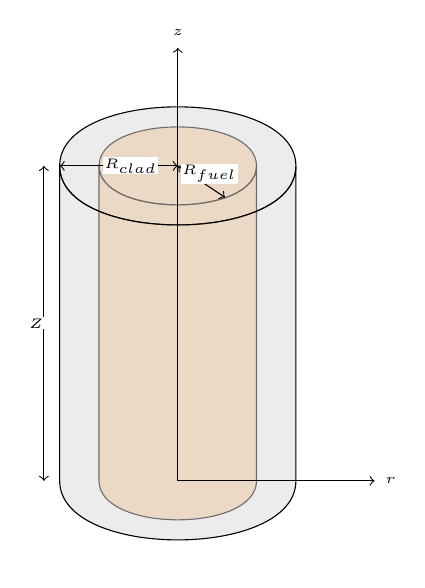
\begin{tikzpicture}

    \tikzstyle{ann} = [fill=white, font=\tiny, inner sep=.5pt]

    % Fuel
    \draw[fill=orange!60, fill opacity=0.5] (0.5,0) to
        [controls=+(90:0.66) and +(90:0.66)] (2.5,0);

    \draw[fill=orange!60, fill opacity=0.5] (0.5,0) .. controls +(-90:0.66)
    and +(-90:0.66) .. (2.5,0);

    \draw[fill=orange!60, fill opacity=0.5] (0.5,0) .. controls +(-90:0.66)
    and +(-90:0.66) .. (2.5,0)
        -- (2.5,-4) .. controls +(-90:0.66) and +(-90:0.66) .. (0.5,-4) -- (0.5,0);


    % Clad
    \draw[fill=lightgray!60, fill opacity=0.5] (0,0) to
        [controls=+(90:1.0) and +(90:1.0)] (3,0);

    \draw[fill=lightgray!60, fill opacity=0.5] (0,0) .. controls +(-90:1.0)
    and +(-90:1.0) .. (3,0);

    \draw[fill=lightgray!60, fill opacity=0.5] (0,0) .. controls +(-90:1.0)
    and +(-90:1.0) .. (3,0)
        -- (3,-4) .. controls +(-90:1.0) and +(-90:1.0) .. (0,-4) -- (0,0);

    % Rfuel and Rclad
    \draw[arrows=<->,line width=.4pt](1.5,0)--(2.1,-.4);
    \draw[arrows=<->,line width=.4pt](1.5,0)--(0,0);
    \node[ann] at (0.9,0) {$R_{clad}$};
    \node[ann] at (1.9,-0.1) {$R_{fuel}$};

    \draw[arrows=<->,line width=.4pt](-0.2,0)--(-0.2,-4);
    \node[ann] at (-0.3,-2) {$Z$};

    % z- and r- axes
    \draw[arrows=->,line width=.4pt](1.5,-4)--(1.5,1.5);
    \draw[arrows=->,line width=.4pt](1.5,-4)--(4.0,-4.0);
    \node[ann] at (1.5,1.7) {$z$};
    \node[ann] at (4.2,-4) {$r$};

    %\node[ann] at (3.5,0.5) {$\Phi=0\mbox{ at }z=Z$};
    %\node[ann] at (3.5,-4.5) {$\Phi=0\mbox{ at }z=0$};

    %\node[ann] at (5.5,-1.3) {$-k_{clad}\nabla T^{clad}
    %                         =h_{conv}(T^{clad}-T_{m})
    %                         \mbox{ at }r=R_{clad}$};
    %\node[ann] at (4.3,-2.8) {$-k_{fuel}\nabla T^{fuel}
    %                           =-k_{clad}\nabla T^{clad}
    %                           =h_{gap}(T^{fuel}-T^{clad})
    %                           \mbox{ at }r=R_{fuel}$};

    %\node[ann] at (3.5,-4.7) {$H=0\mbox{ at }z=0$};

\end{tikzpicture}


  \end{column}

  \begin{column}{7cm}
    \tiny

    \begin{block}{Neutronics - multigroup diffusion equation}
      \begin{align}
        \left( \frac{1}{v^{g}} \partial_{t} 
        - \nabla \cdot D^{g} \nabla
        + \Sigma_{r}^{g} \right) \Phi^{g}
        = \frac{1}{\lambda} \chi^{g} \sum_{g'} \nu \Sigma_{f}^{g'} \Phi^{g'}
        + \sum_{g'\neq g} \Sigma_{s}^{g' \rightarrow g} \Phi^{g'}
        \nonumber 
      \end{align}
    \end{block}

    \begin{block}{Heat transfer  - heat conduction equation}
      \begin{align}
        \left( \rho C_{p} \partial_{t}
        - \nabla \cdot k \nabla \right) T 
        = q''' \nonumber
      \end{align}
    \end{block}
 
    \begin{block}{Fluid dynamics  - enthalpy balance}
      \begin{align}
        \left( \partial_{t}
        - \nabla \cdot \bs{u} \right) \rho_m H 
        = - \nabla \varphi \nonumber
      \end{align}
    \end{block}

  \end{column}
  \end{columns}

\end{frame}

